\section{Tutash idishlar}

\begin{enumerate}

\item Tutash idishlar bitta tirsagida simob ustuni 16 cm. Ikkinchi tirsakdagi kerosin ustunining balandligi necha metr? Simobning zichligi 13,6 g/cm$^3$, kerosinniki 0,8 g/cm$^3$ ga teng.

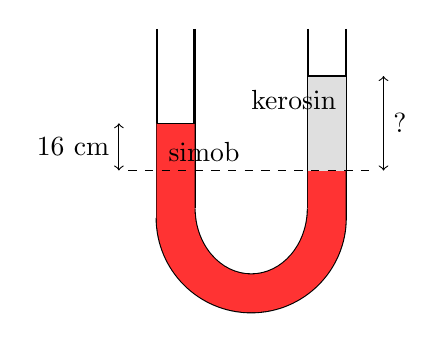
\begin{tikzpicture}[scale=0.6]

% ---- idish devorlari ----
\draw[thick] (-2,5) -- (-2,1);
\draw[thick] (-1.2,5) -- (-1.2,1.2);
\draw[thick] ( 2,5) -- ( 2,1);
\draw[thick] ( 1.2,5) -- ( 1.2,1.2);
\draw[thick] (-2,1) arc (180:360:2 and 2);
\draw[thick] (-1.2,1.2) arc (180:360:1.2 and 1.4);

% ---- simob ----
\fill[red!80]
(-2,3) -- (-1.2,3)
-- (-1.2,1.2)
arc (180:360:1.2 and 1.4) -- (1.2,2)--(2,2) -- (2,1)
arc (360:180:2 and 2)
-- cycle;

% ---- kerosin ----
\fill[gray!25] (1.2,2) rectangle (2,4);

% ---- sath chiziqlari ----
\draw (-2,3) -- (-1.2,3);
\draw (1.2,4) -- (2,4);

% ---- dashed reference ----
\draw[dashed] (-2.6,2) -- (2.6,2);

% ---- 16 cm ----
\draw[<->] (-2.8,2) -- (-2.8,3);
\node[left] at (-2.8,2.5) {16 cm};

% ---- ? ----
\draw[<->] (2.8,2) -- (2.8,4);
\node[right] at (2.8,3) {?};

% ---- labels ----
\node at (-1,2.4) {simob};
\node at (0.9,3.5) {kerosin};

\end{tikzpicture}

\begin{enumerate}[label=\Alph*)]
\item 1,36
\item 2,72
\item 13,6
\item 16
\end{enumerate}


\item Tutash idishlarning biriga suv, ikkinchisiga kerosin solingan. 
Suv ustunining balandligi 16 cm bo‘lsa, kerosin ustunining balandligini 
(cm) toping. Suvning zichligi 1 g/cm$^3$, kerosinniki 0,8 g/cm$^3$ ga teng.

\begin{enumerate}[label=\Alph*)]
\item 18
\item 16
\item 24
\item 20
\end{enumerate}


\item Tutash idish naylaridan biriga simob quyilgan. Ikkinchi nayda suv bor. 
Simob ustunining balandligi 5 cm. Simob va suv ustunlari muvozanatda 
turgan bo‘lsa, suv ustunining balandligi necha cm?

\begin{enumerate}[label=\Alph*)]
\item 13,6
\item 68
\item 75
\item 100
\end{enumerate}


\item U–simon tutash idishga suv va kerosin quyilgan. Suv sathi idishning yuqori uchidan 30 cm pastda joylashgan. Idishning narigi tirsagi kerosin bilan to‘ldirilgan. Kerosin ustunining balandligini toping (cm).

\begin{enumerate}[label=\Alph*)]
\item 50
\item 60
\item 120
\item 150
\end{enumerate}


\item U-simon tutash idishning ikkinchi tirsagi radiusi birinchisinikidan 
2 marta katta. Unga suyuqlik quyilsa, birinchi va ikkinchi tirsaklardagi 
suyuqlik ustunlarining balandliklari nisbati $h_1/h_2$ qanday bo‘ladi?

\begin{enumerate}[label=\Alph*)]
\item 2
\item 4
\item $\dfrac14$
\item 1
\end{enumerate}


\item U-simon (tutash) idishga quyilgan va bir-biri bilan aralashmaydigan ikki xil suyuqliklarning ajralish sathidan boshlanadigan balandliklarining nisbati $\frac{h_1}{h_2}=2$ bo‘lsa, bu suyuqliklarning zichliklari nisbati 
$\frac{\rho_1}{\rho_2}$ qanday?

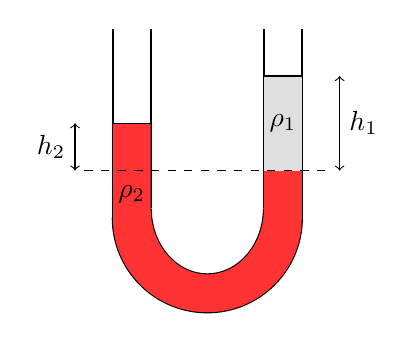
\begin{tikzpicture}[scale=0.6]

% ---- idish devorlari ----
\draw[thick] (-2,5) -- (-2,1);
\draw[thick] (-1.2,5) -- (-1.2,1.2);
\draw[thick] ( 2,5) -- ( 2,1);
\draw[thick] ( 1.2,5) -- ( 1.2,1.2);
\draw[thick] (-2,1) arc (180:360:2 and 2);
\draw[thick] (-1.2,1.2) arc (180:360:1.2 and 1.4);

% ---- simob ----
\fill[red!80]
(-2,3) -- (-1.2,3)
-- (-1.2,1.2)
arc (180:360:1.2 and 1.4) -- (1.2,2)--(2,2) -- (2,1)
arc (360:180:2 and 2)
-- cycle;

% ---- kerosin ----
\fill[gray!25] (1.2,2) rectangle (2,4);

% ---- sath chiziqlari ----
\draw (-2,3) -- (-1.2,3);
\draw (1.2,4) -- (2,4);

% ---- dashed reference ----
\draw[dashed] (-2.6,2) -- (2.6,2);

% ---- 16 cm ----
\draw[<->] (-2.8,2) -- (-2.8,3);
\node[left] at (-2.8,2.5) {$h_2$};

% ---- ? ----
\draw[<->] (2.8,2) -- (2.8,4);
\node[right] at (2.8,3) {$h_1$};

% ---- labels ----
\node at (1.6,3) {$\rho_1$};
\node at (-1.6,1.5) {$\rho_2$};

\end{tikzpicture}

\begin{enumerate}[label=\Alph*)]
\item 0,5
\item 0,25
\item 1
\item 2
\end{enumerate}


\item Tutash idishda dastlab suv va simob bor edi. Suv ustunining balandligi 68 cm. Simob idishning ikkala qismida bir xil balandlikka ega bo‘lishi uchun idishning ikkinchi tomoniga necha cm balandlikkacha kerosin quyish kerak?

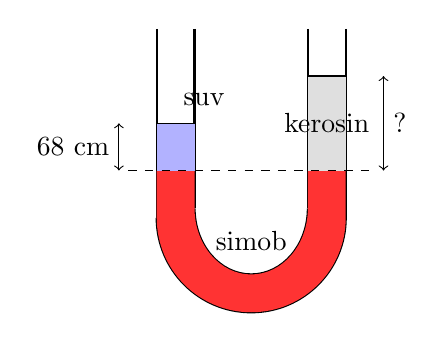
\begin{tikzpicture}[scale=0.6]

% ---- idish devorlari ----
\draw[thick] (-2,5) -- (-2,1);
\draw[thick] (-1.2,5) -- (-1.2,1.2);
\draw[thick] ( 2,5) -- ( 2,1);
\draw[thick] ( 1.2,5) -- ( 1.2,1.2);
\draw[thick] (-2,1) arc (180:360:2 and 2);
\draw[thick] (-1.2,1.2) arc (180:360:1.2 and 1.4);

% ---- simob ----
\fill[red!80]
(-2,2) -- (-1.2,2)
-- (-1.2,1.2)
arc (180:360:1.2 and 1.4) -- (1.2,2)--(2,2) -- (2,1)
arc (360:180:2 and 2)
-- cycle;

% ---- kerosin ----
\fill[gray!25] (1.2,2) rectangle (2,4);
\fill[blue!30] (-2,2) rectangle (-1.2,3);

% ---- sath chiziqlari ----
\draw (-2,3) -- (-1.2,3);
\draw (1.2,4) -- (2,4);

% ---- dashed reference ----
\draw[dashed] (-2.6,2) -- (2.6,2);

% ---- 16 cm ----
\draw[<->] (-2.8,2) -- (-2.8,3);
\node[left] at (-2.8,2.5) {68 cm};

% ---- ? ----
\draw[<->] (2.8,2) -- (2.8,4);
\node[right] at (2.8,3) {?};

% ---- labels ----
\node at (1.6,3) {kerosin};
\node at (-1,3.5) {suv};
\node at (-0,0.5) {simob};

\end{tikzpicture}

\begin{enumerate}[label=\Alph*)]
\item 15
\item 53
\item 68
\item 85
\end{enumerate}


\item Tutash idishlarga simob, kerosin va $x$ suyuqlik rasmdagi kabi quyilgan. $x$ suyuqlikning zichligini toping (kg/m$^3$).

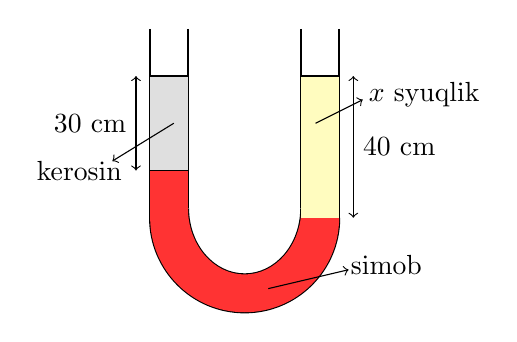
\begin{tikzpicture}[scale=0.6]

% ---- idish devorlari ----
\draw[thick] (-2,5) -- (-2,1);
\draw[thick] (-1.2,5) -- (-1.2,1.2);
\draw[thick] ( 2,5) -- ( 2,1);
\draw[thick] ( 1.2,5) -- ( 1.2,1.2);
\draw[thick] (-2,1) arc (180:360:2 and 2);
\draw[thick] (-1.2,1.2) arc (180:360:1.2 and 1.4);

% ---- simob ----
\fill[red!80]
(-2,2) -- (-1.2,2)
-- (-1.2,1.2)
arc (180:360:1.2 and 1.4) -- (1.2,1)--(2,1) -- (2,1)
arc (360:180:2 and 2)
-- cycle;

% ---- kerosin ----
\fill[yellow!25] (1.2,1) rectangle (2,4);
\fill[gray!25] (-2,2) rectangle (-1.2,4);

% ---- sath chiziqlari ----
\draw (-2,2) -- (-1.2,2);
\draw (-2,4) -- (-1.2,4);
\draw (1.2,4) -- (2,4);


% ---- 16 cm ----
\draw[<->] (-2.3,2) -- (-2.3,4);
\node[left] at (-2.3,3) {30 cm};

% ---- ? ----
\draw[<->] (2.3,1) -- (2.3,4);
\node[right] at (2.3,2.5) {40 cm};

% ---- labels ----
\node at (3.8,3.6) {$x$ syuqlik};
\draw[->] (1.5,3) -- (2.5,3.5);
\node at (-3.5,2) {kerosin};
\draw[->] (-1.5,3) -- (-2.8,2.2);
\node at (3,0) {simob};
\draw[->] (0.5,-0.5) -- (2.2,-0.1);

\end{tikzpicture}

\begin{enumerate}[label=\Alph*)]
\item 2500
\item 5300
\item 7800
\item 4000
\end{enumerate}


\item Tutash idishlarga simob quyilgan (1-rasm). $S_1=10$ cm$^2$ yuzali tirsakka $m=204$ g massali suv quyildi (2-rasm). $S_2=5$ cm$^2$ yuzali tirsakda simob qancha $h$ balandlikka ko‘tariladi (cm)?

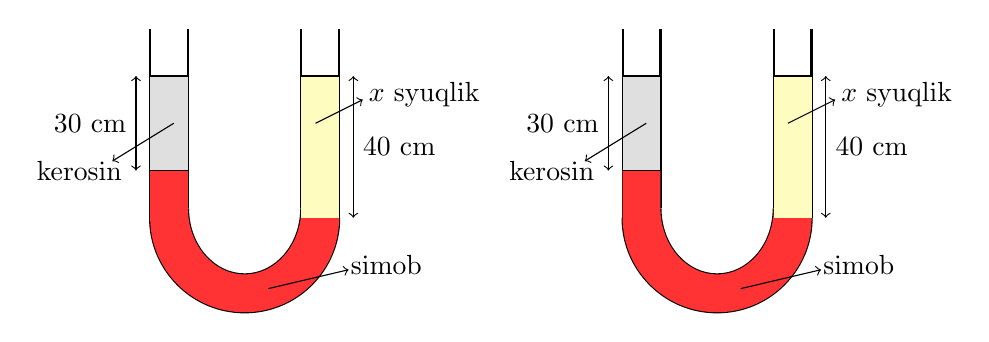
\begin{tikzpicture}[scale=0.6]

% ---- idish devorlari ----
\draw[thick] (-2,5) -- (-2,1);
\draw[thick] (-1.2,5) -- (-1.2,1.2);
\draw[thick] ( 2,5) -- ( 2,1);
\draw[thick] ( 1.2,5) -- ( 1.2,1.2);
\draw[thick] (-2,1) arc (180:360:2 and 2);
\draw[thick] (-1.2,1.2) arc (180:360:1.2 and 1.4);

% ---- simob ----
\fill[red!80]
(-2,2) -- (-1.2,2)
-- (-1.2,1.2)
arc (180:360:1.2 and 1.4) -- (1.2,1)--(2,1) -- (2,1)
arc (360:180:2 and 2)
-- cycle;

% ---- kerosin ----
\fill[yellow!25] (1.2,1) rectangle (2,4);
\fill[gray!25] (-2,2) rectangle (-1.2,4);

% ---- sath chiziqlari ----
\draw (-2,2) -- (-1.2,2);
\draw (-2,4) -- (-1.2,4);
\draw (1.2,4) -- (2,4);


% ---- 16 cm ----
\draw[<->] (-2.3,2) -- (-2.3,4);
\node[left] at (-2.3,3) {30 cm};

% ---- ? ----
\draw[<->] (2.3,1) -- (2.3,4);
\node[right] at (2.3,2.5) {40 cm};

% ---- labels ----
\node at (3.8,3.6) {$x$ syuqlik};
\draw[->] (1.5,3) -- (2.5,3.5);
\node at (-3.5,2) {kerosin};
\draw[->] (-1.5,3) -- (-2.8,2.2);
\node at (3,0) {simob};
\draw[->] (0.5,-0.5) -- (2.2,-0.1);


\begin{scope}[xshift=10cm]
% ---- idish devorlari ----
\draw[thick] (-2,5) -- (-2,1);
\draw[thick] (-1.2,5) -- (-1.2,1.2);
\draw[thick] ( 2,5) -- ( 2,1);
\draw[thick] ( 1.2,5) -- ( 1.2,1.2);
\draw[thick] (-2,1) arc (180:360:2 and 2);
\draw[thick] (-1.2,1.2) arc (180:360:1.2 and 1.4);

% ---- simob ----
\fill[red!80]
(-2,2) -- (-1.2,2)
-- (-1.2,1.2)
arc (180:360:1.2 and 1.4) -- (1.2,1)--(2,1) -- (2,1)
arc (360:180:2 and 2)
-- cycle;

% ---- kerosin ----
\fill[yellow!25] (1.2,1) rectangle (2,4);
\fill[gray!25] (-2,2) rectangle (-1.2,4);

% ---- sath chiziqlari ----
\draw (-2,2) -- (-1.2,2);
\draw (-2,4) -- (-1.2,4);
\draw (1.2,4) -- (2,4);


% ---- 16 cm ----
\draw[<->] (-2.3,2) -- (-2.3,4);
\node[left] at (-2.3,3) {30 cm};

% ---- ? ----
\draw[<->] (2.3,1) -- (2.3,4);
\node[right] at (2.3,2.5) {40 cm};

% ---- labels ----
\node at (3.8,3.6) {$x$ syuqlik};
\draw[->] (1.5,3) -- (2.5,3.5);
\node at (-3.5,2) {kerosin};
\draw[->] (-1.5,3) -- (-2.8,2.2);
\node at (3,0) {simob};
\draw[->] (0.5,-0.5) -- (2.2,-0.1);

\end{scope}

\end{tikzpicture}

\begin{enumerate}[label=\Alph*)]
\item 2,5
\item 2
\item 1
\item 1,5
\end{enumerate}
\end{enumerate}




\begin{table}[h!]
\centering
\begin{tabular}{|c|c|c|c|c|c|c|}
\hline
№ & J. & № & J. & № & J.  \\ \hline
1 & B & 6 & A & 11 &  \\ \hline
2 & D & 7 & D & 12 &  \\ \hline
3 & B & 8 & D & 13 &  \\ \hline
4 & A & 9 & C & 14 &   \\ \hline
5 & D & 10 &  & 15 &   \\ \hline
\end{tabular}
\end{table}